\chapter{SPT-DSFG SEDs}

\begin{figure}
	\centering
	\caption[SEDs of SPT sample (Optically thin)]{SEDs of SPT sample (Optically thin).}
	\includegraphics[width=\columnwidth]{Figures/spt_ot_SEDs_1.pdf}
\end{figure}
\begin{figure}
	\centering
	\includegraphics[width=\columnwidth]{Figures/spt_ot_SEDs_2.pdf}
\end{figure}
\begin{figure}
	\centering
	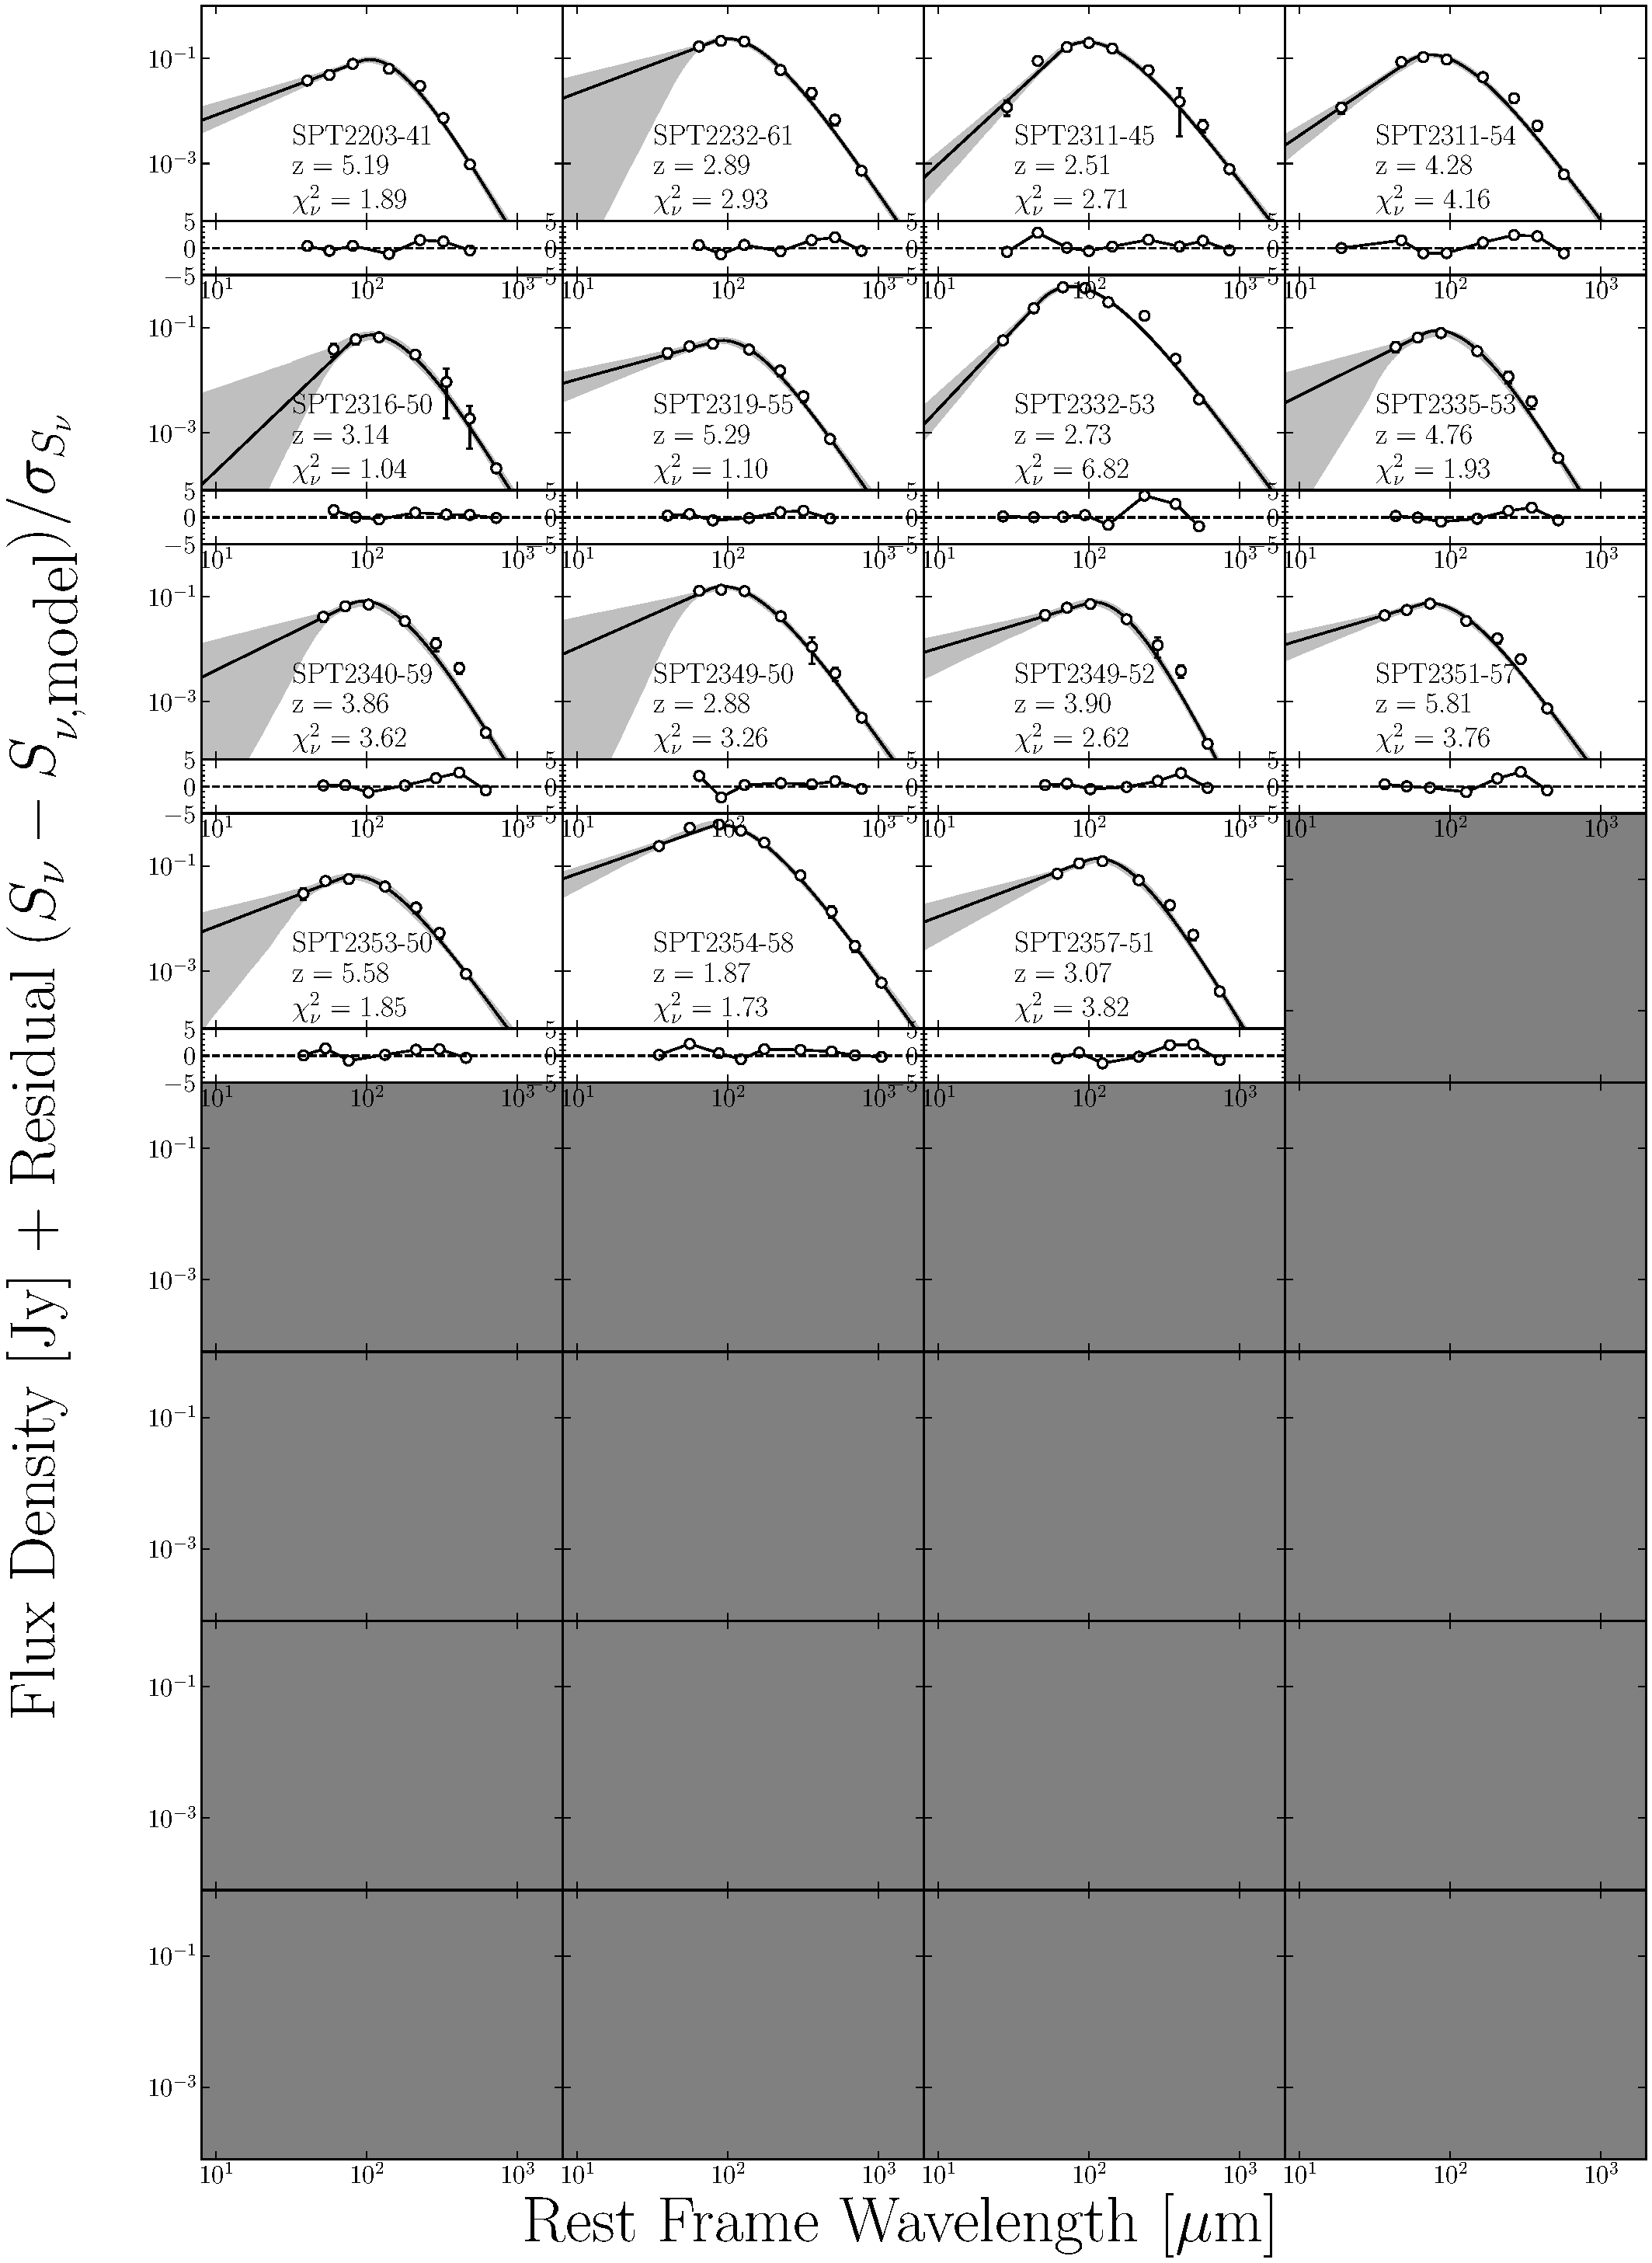
\includegraphics[width=\columnwidth]{Figures/spt_ot_SEDs_3.pdf}
\end{figure}


\begin{figure}
	\centering
	\caption[SEDs of SPT sample ($\lambda_1 = 100\,\mu$m)]{SEDs of SPT sample ($\lambda_1 = 100\,\mu$m).}
	\includegraphics[width=\columnwidth]{Figures/spt_go100_SEDs_1.pdf}
\end{figure}
\begin{figure}
	\centering
	\includegraphics[width=\columnwidth]{Figures/spt_go100_SEDs_2.pdf}
\end{figure}
\begin{figure}
	\centering
	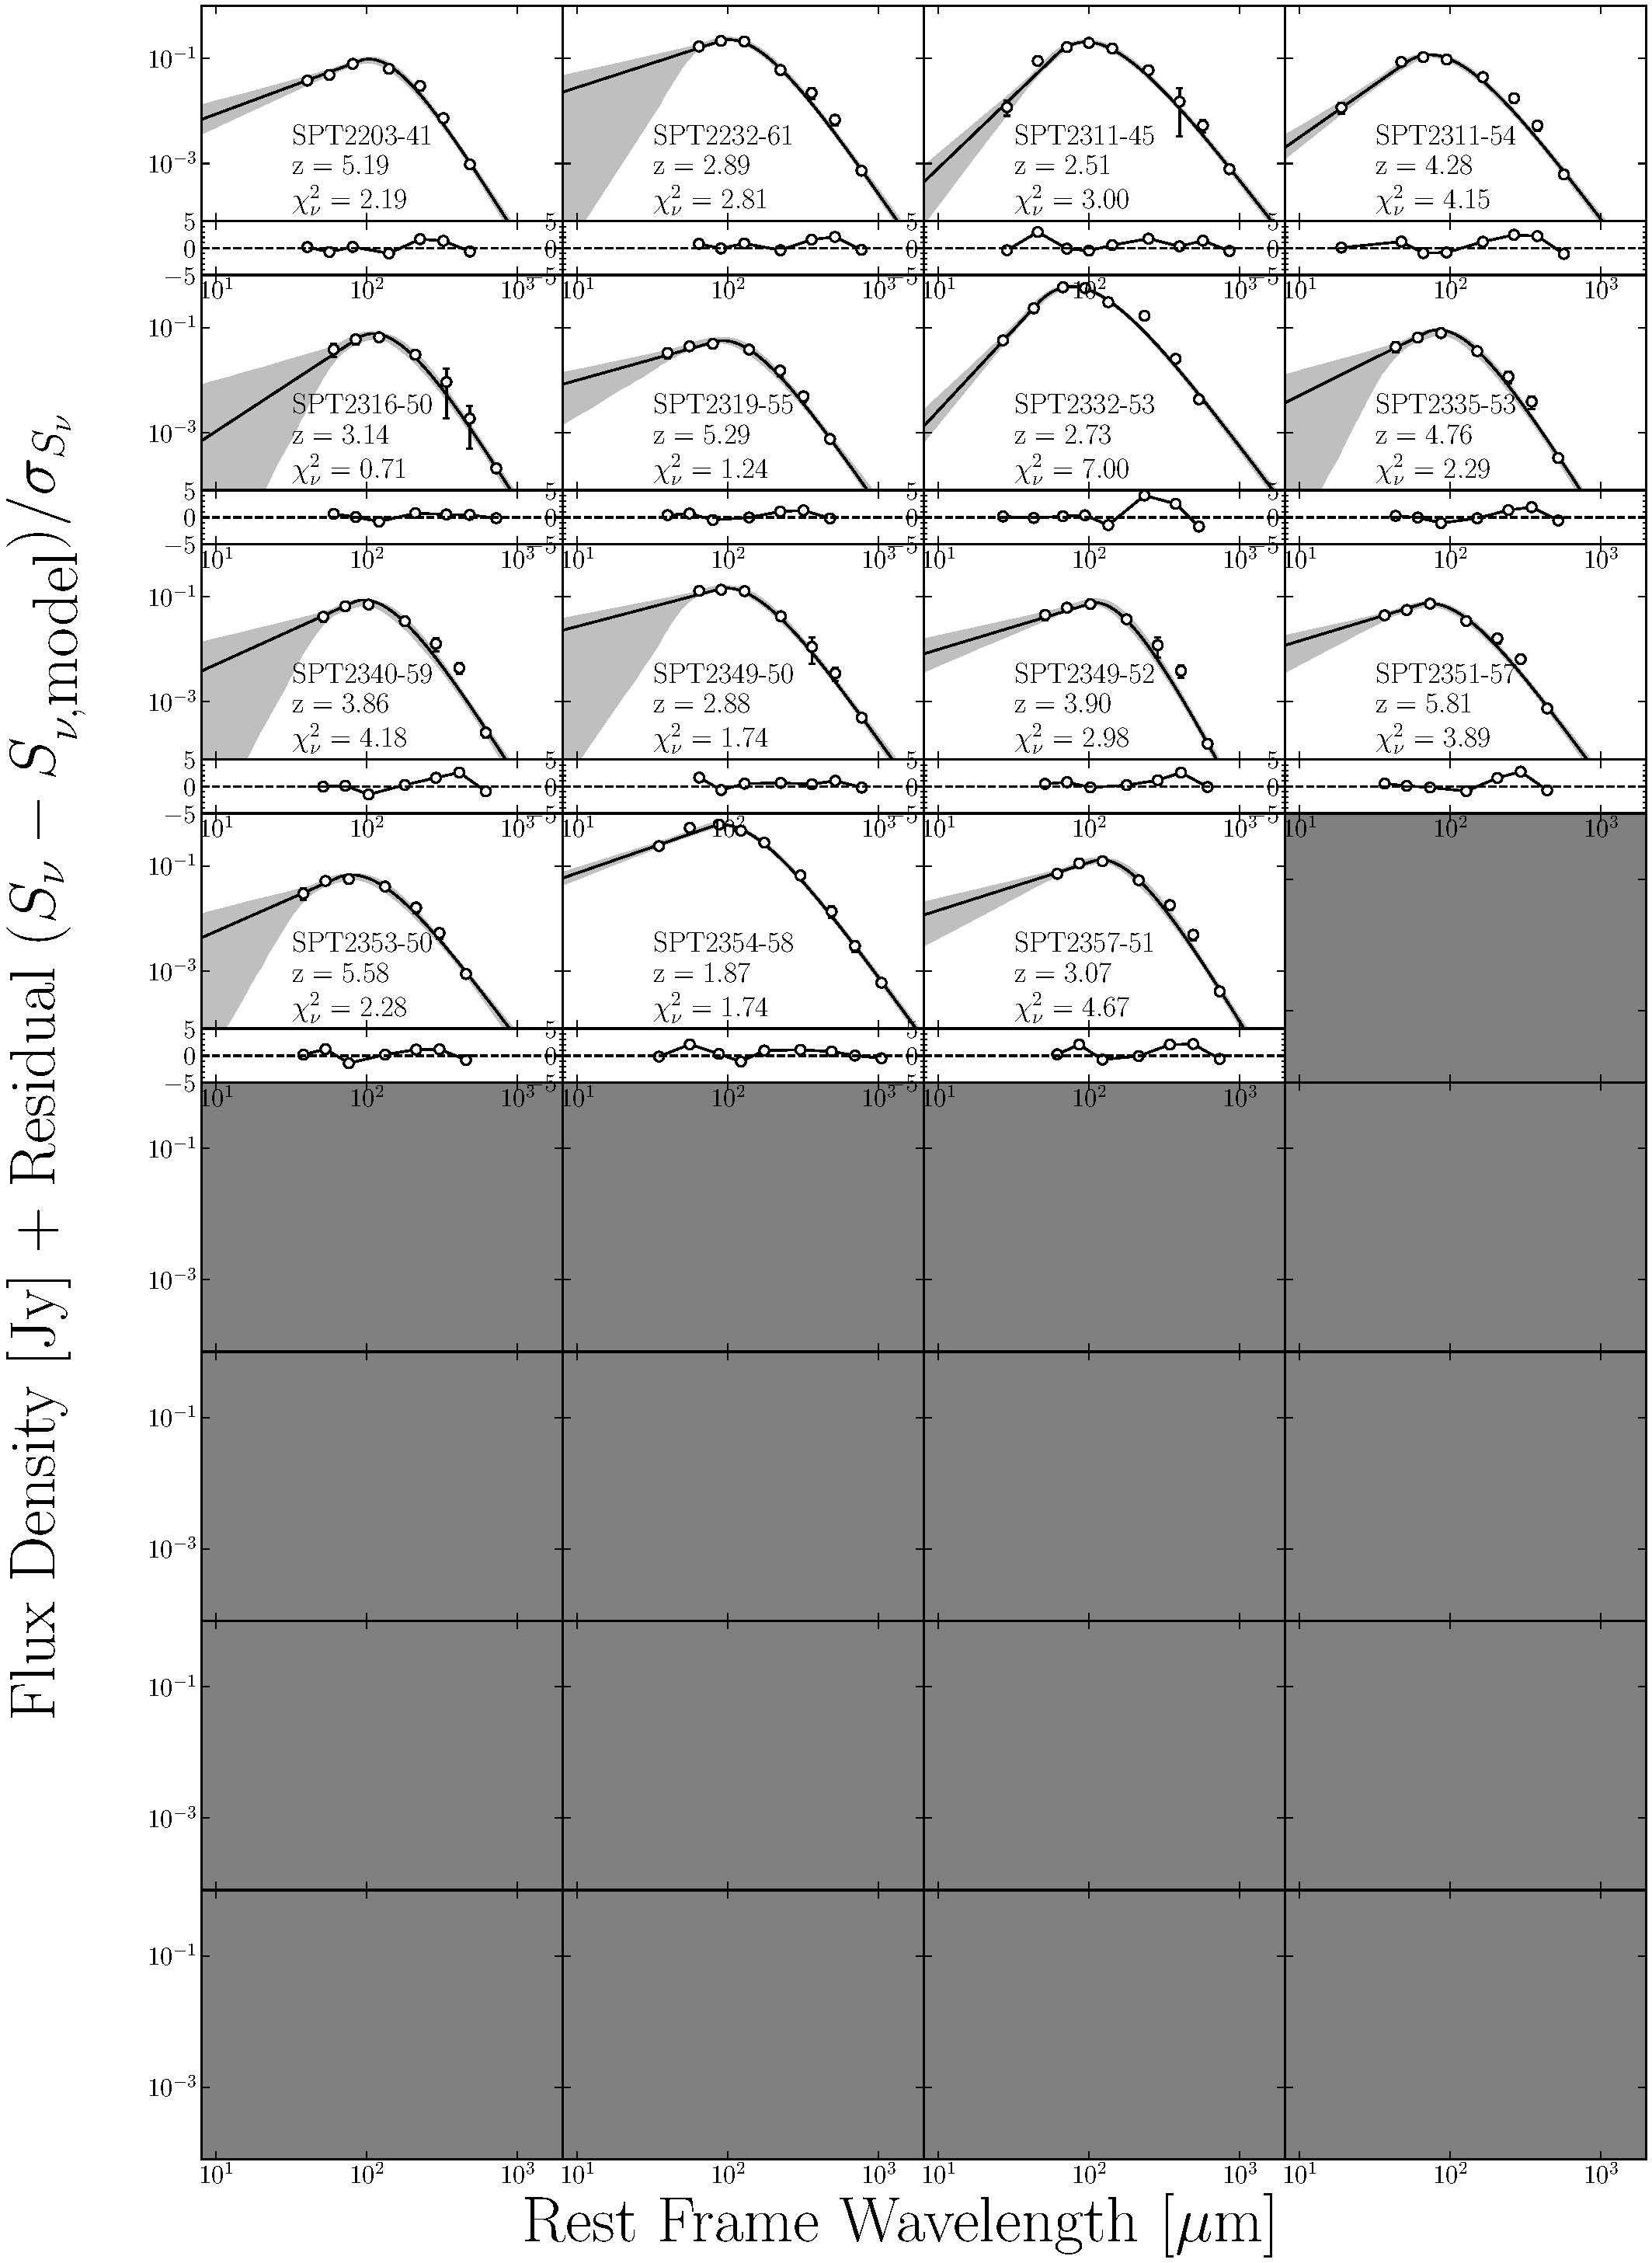
\includegraphics[width=\columnwidth]{Figures/spt_go100_SEDs_3.pdf}
\end{figure}


\begin{figure}
	\centering
	\caption[SEDs of SPT sample ($\lambda_1 = 200\,\mu$m)]{SEDs of SPT sample ($\lambda_1 = 200\,\mu$m).}
	\includegraphics[width=\columnwidth]{Figures/spt_go200_SEDs_1.pdf}
\end{figure}
\begin{figure}
	\centering
	\includegraphics[width=\columnwidth]{Figures/spt_go200_SEDs_2.pdf}
\end{figure}
\begin{figure}
	\centering
	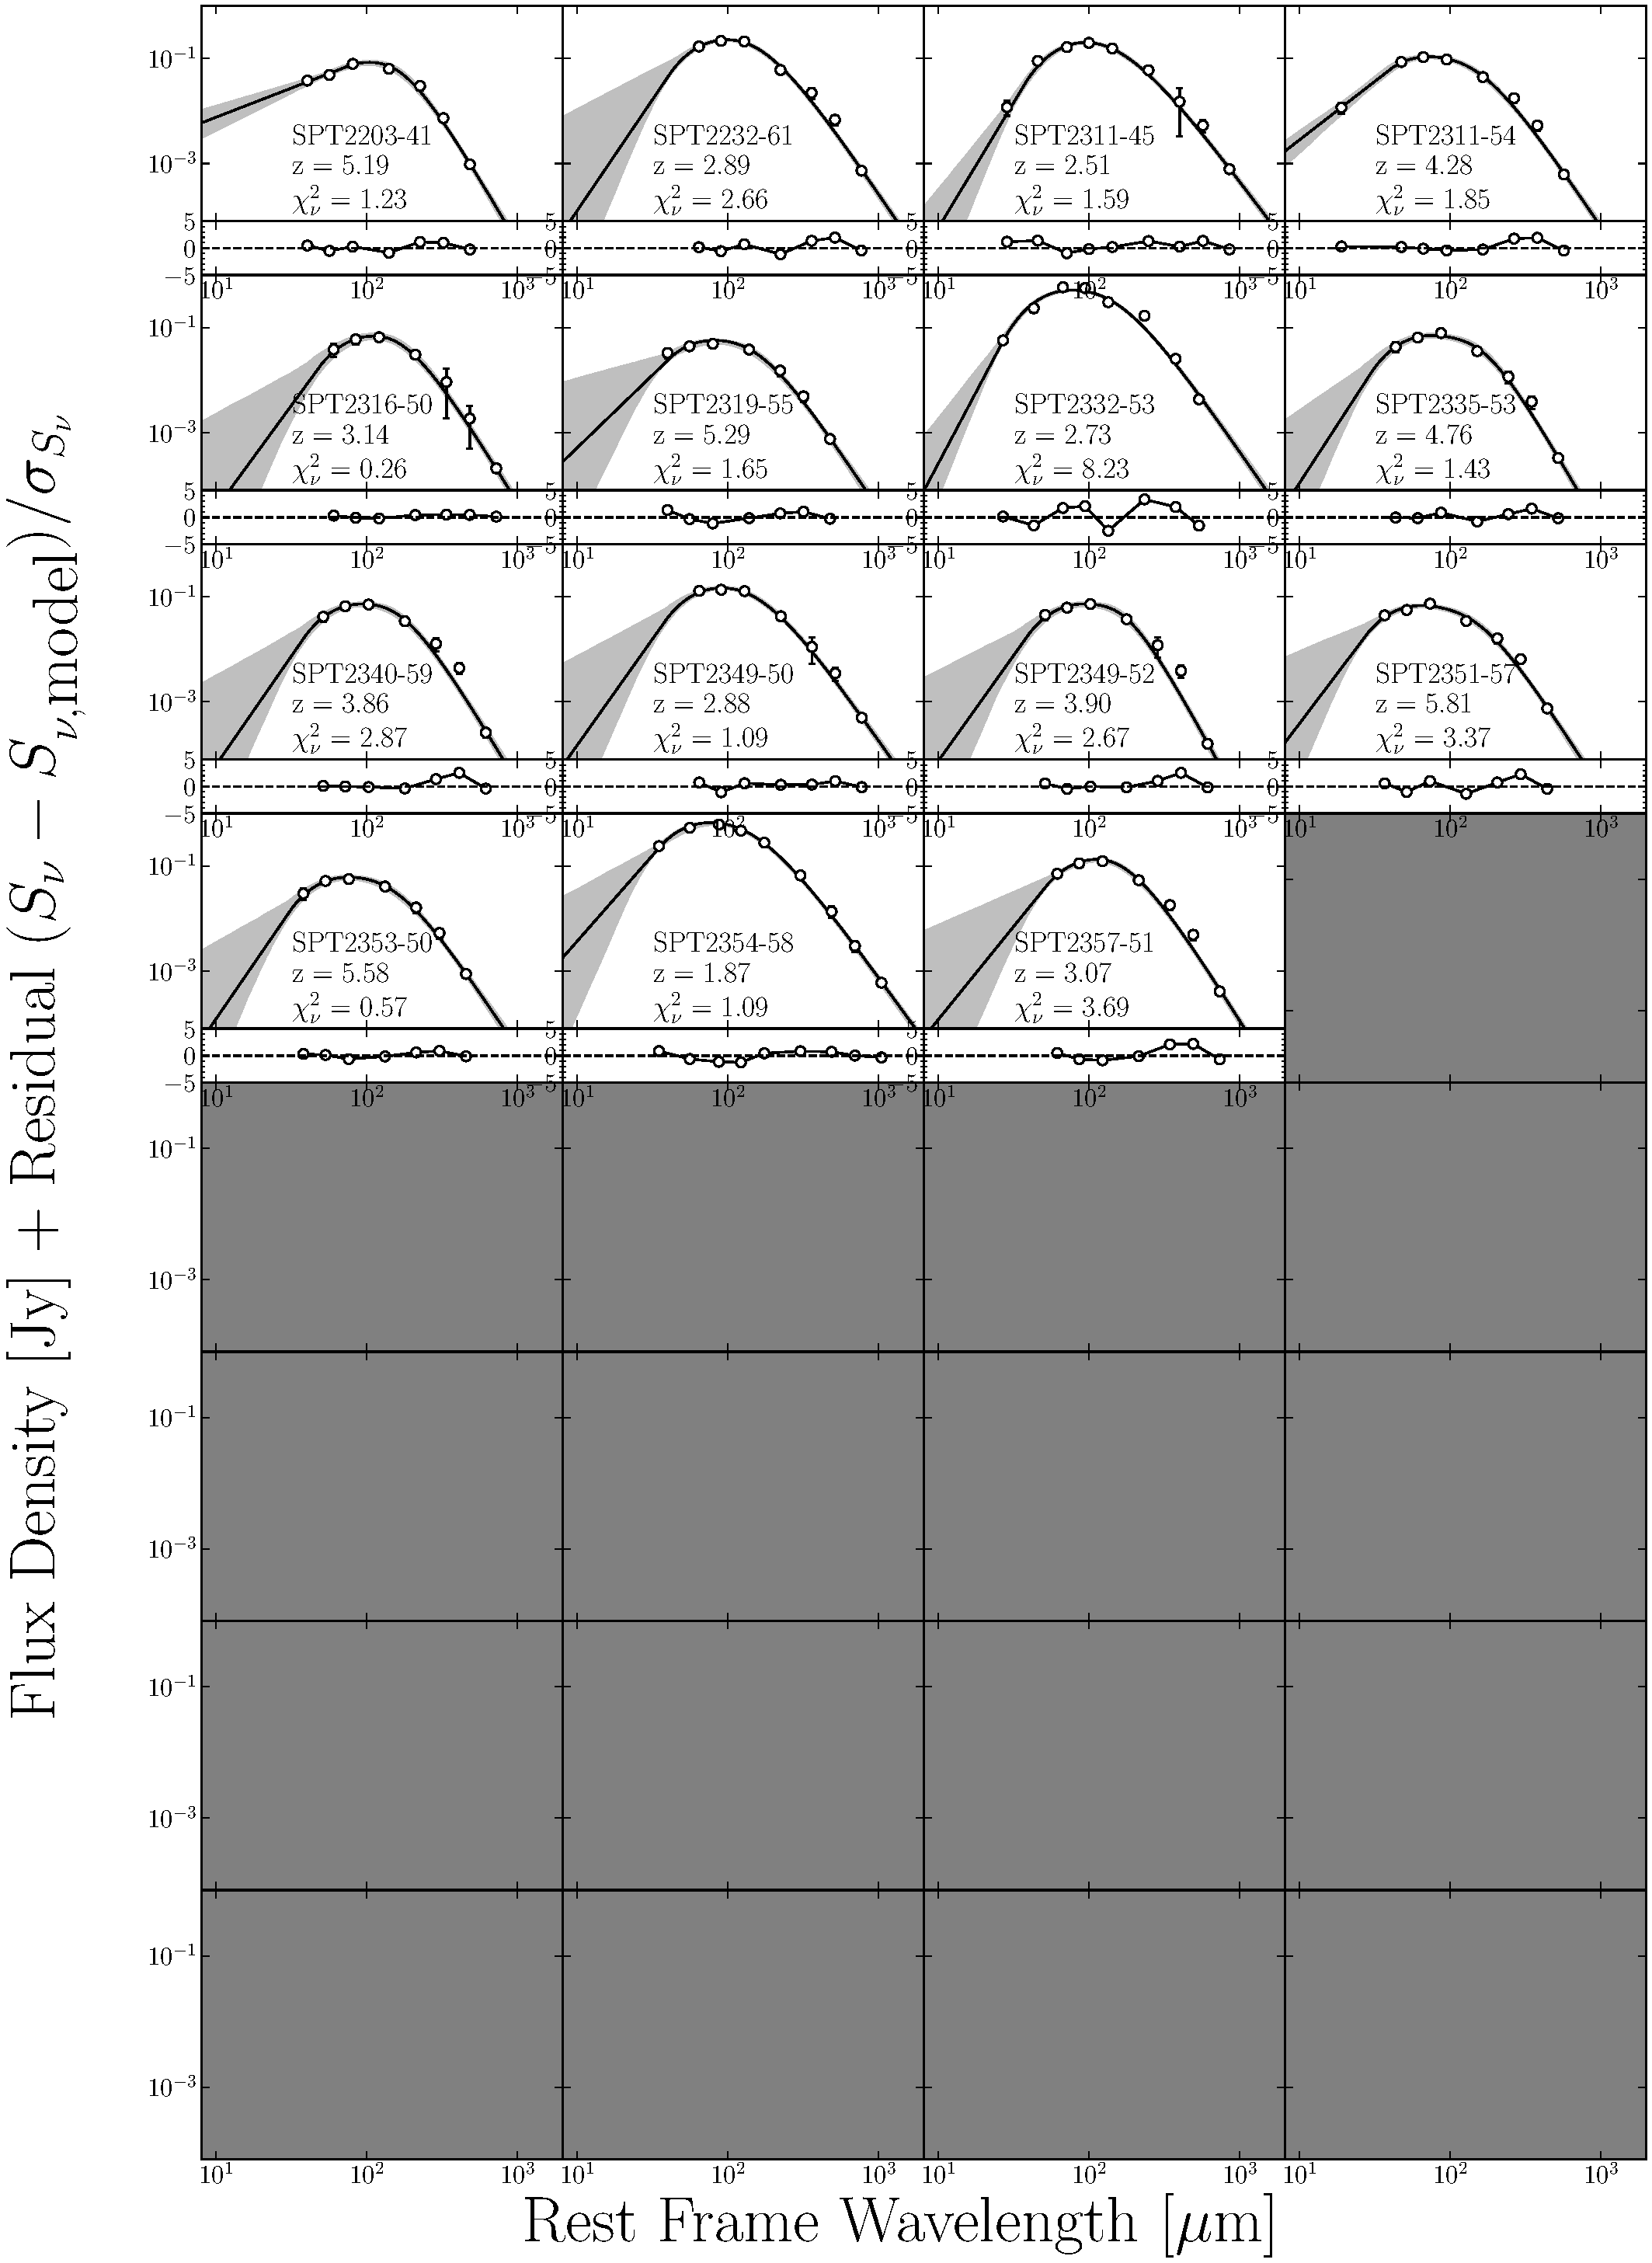
\includegraphics[width=\columnwidth]{Figures/spt_go200_SEDs_3.pdf}
\end{figure}
